\section{Introduction to popular distributions and their properties}
\begin{itemize}
	\item This section (lecture 1 and 2) reviews different kinds of distributions, including the exponential family, Student-t distribution and common distributions for binary and discrete variables
	\item Furthermore, we shortly introduce Independent Component Analysis and Information theory
	\item In general, the first two lectures gave some fundamental knowledge we will use a couple of times for the rest of the course
	\item More mathematical tricks or examples of the exponential family can be found in the appendix
\end{itemize}
\subsection{Exponential family distributions}
\textbf{(Bishop 2.4)}
\begin{itemize}
	\item A distribution is considered a member of the exponential family if it can be written as follows:
	\begin{equation*}
	\tcbox[nobeforeafter]{\(
		\begin{split}
			p(\bm{x}|\bm{\eta}) & = h(\bm{x})g(\bm{\eta})\exp\left(\bm{\eta}^T \cdot \bm{u}(\bm{x})\right)\\[5pt]
			\bm{\eta} & \hspace{3mm}\text{natural parameters}\\
			\bm{u}(\bm{x}) & \hspace{3mm}\text{sufficient statistics}\\
		\end{split}
	\)}
	\end{equation*}
	\item $\bm{u}(\bm{x})$ is called sufficient statistics because for the maximum likelihood estimate of $\bm{\eta}$, it is sufficient to record $\sum_{n=1}^{N}\bm{u}(\bm{x}_n)$ instead of the whole dataset $\left\{\bm{x}_n\right\}_{n=1}^{N}$ (see below for ML estimate)
	\item An important property of the exponential families is that the moments of distributions (i.e. mean and variance) can be determined by deriving $-\ln g(\bm{\eta})$ by $\bm{\eta}$:
	\begin{equation*}
		\begin{split}
			\text{Normalization constant}\hspace{2mm} z(\bm{\eta}) & = \frac{1}{g(\bm{\eta})} = \int h(\bm{x})\exp\left(\bm{\eta}^T \cdot \bm{u}(\bm{x})\right) d\bm{x}\\
			\frac{\partial}{\partial \bm{\eta}} -\ln g(\bm{\eta}) & = -\frac{1}{z(\bm{\eta})} \int h(\bm{x})\bm{u}(\bm{x})\exp\left(\bm{\eta}^T \cdot \bm{u}(\bm{x})\right) d\bm{x} = \E[\bm{u}(\bm{x})\vert \bm{\eta}]\\
		\end{split}
	\end{equation*}
	\begin{itemize}
		\item Note that these moments are of the sufficient statistics $\bm{u}(\bm{x})$, and not $\bm{x}$
		\item Additionally, the second moment around the mean can be determined by: $\nabla_{\bm{\eta}}^2 -\ln g(\bm{\eta})$
	\end{itemize}
	\item From the first moment, we can show that the \underline{MLE solution} of the natural parameters are:
	$$\tcbox[nobeforeafter]{\(-\nabla_{\bm{\eta}}\ln g(\bm{\eta}) = \E[\bm{u}(\bm{x})\vert \bm{\eta}] \implies -\nabla_{\bm{\eta}}\ln g(\bm{\eta}_{\text{ML}}) = \frac{1}{N}\sum_{n=1}^{N} \bm{u}(\bm{x})\)}$$
\end{itemize}
\subsubsection{Conjugate priors}
\begin{itemize}
	\item A conjugate prior $p(\bm{\eta})$ is conjugate to the likelihood so that the posterior $p(\bm{\eta}|\bm{X})$ has the same form as the prior
	\item Each member of the exponential family has a conjugate prior
	\item To find the conjugate prior for a exponential distribution as likelihood, we only have to look at $\bm{\eta}$ of the likelihood and $\bm{u}(\bm{x})$ of the prior take on the same form. Then, we simply get:
	\begin{equation*}
		\begin{split}
			\bm{u}(\bm{x})_{\text{posterior}} & = \bm{\eta}_{\text{likelihood}} = \bm{u}(\bm{x})_{\text{prior}}\\
			\bm{\eta}_{\text{posterior}} & = \bm{u}(\bm{x})_{\text{likelihood}} + \bm{\eta}_{\text{prior}}
		\end{split}
	\end{equation*}
\end{itemize}
\subsubsection{Bayesian Inference for Gaussian}
\begin{itemize}
	\item We can demonstrate the conjugate prior idea for Gaussians (one dimensional), where we have to distinguish three cases
\end{itemize}
\begin{enumerate}
	\item \underline{Variance known, mean estimated}
	\begin{itemize}
		\item Conjugate prior is a Gaussian $p(\mu)=\mathcal{N}(\mu\vert\mu_0, \sigma_0^2)$ such that our posterior has the distribution:
		\begin{equation*}
		\tcbox[nobeforeafter]{\(
			\begin{split}
				& \textbf{Variance known, mean estimated}\\
				& p(\mu|\mathcal{D})=\mathcal{N}(\mu|\mu_N, \sigma_N^2), \hspace{5mm}\mu_N= \frac{\sigma^2 \mu_0 + N\sigma_0^2 \mu_{\text{ML}}}{N\sigma_0^2 + \sigma^2}, \hspace{5mm}\frac{1}{\sigma_N^2}=\frac{1}{\sigma_0^2} + \frac{N}{\sigma^2}
			\end{split}
		\)}
		\end{equation*}
	\end{itemize}
	\item \underline{Mean unknown, variance estimated}
	\begin{itemize}
		\item Conjugate prior for the precision $\lambda=\frac{1}{\sigma^2}$ is a Gamma distribution $\text{Gamma}(\lambda|a_0, b_0)$ such that the posterior is:
		\begin{equation*}
		\tcbox[nobeforeafter]{\(
			\begin{split}
			& \textbf{Mean known, variance estimated}\\
			& p(\lambda|\mathcal{D})=\text{Gamma}(\lambda|a_N,b_N), \hspace{5mm}a_N=a_0+\frac{N}{2},\hspace{5mm}b_N = b_0+\frac{1}{2}\sum_n(x_n-\mu)^2
			\end{split}
			\)}
		\end{equation*}
	\end{itemize}
	\item \underline{Variance and mean estimated}
	\begin{itemize}
		\item If both are unknown, we have a ``normal-Gamma'' distribution as prior and posterior: $p(\mu,\lambda|a,b,\mu_0, \beta)=\mathcal{N}(\mu|\mu_0, (\beta \lambda^{-1}))\text{Gamma}(\lambda|a,b)$
		\item Finding the posterior is harder in this case because of the combined distribution. For details, see Bishop, but in the lecture it was not further discussed
	\end{itemize}
\end{enumerate}
\subsection{Student's-t distribution}
\begin{itemize}
	\item The Student-t distribution is "heavy-tailed", meaning that the probability for data points decreases slower with the distance from the mean/center than for a Gaussian (polynomial $\text{St}(x)\propto |x|^{-\alpha}$ instead of exponential $\mathcal{N}\propto e^{-\frac{x^2}{\sigma^2}}$)
	\item This makes the distribution more \underline{robust against outliers} as the MLE solution is less influenced by those and focuses more on the biggest data point mass (see Figure~\ref{fig:exponential_families_student_t})
	\begin{figure}[ht!]
		\centering
		\begin{subfigure}{0.25\textwidth}
			\centering
			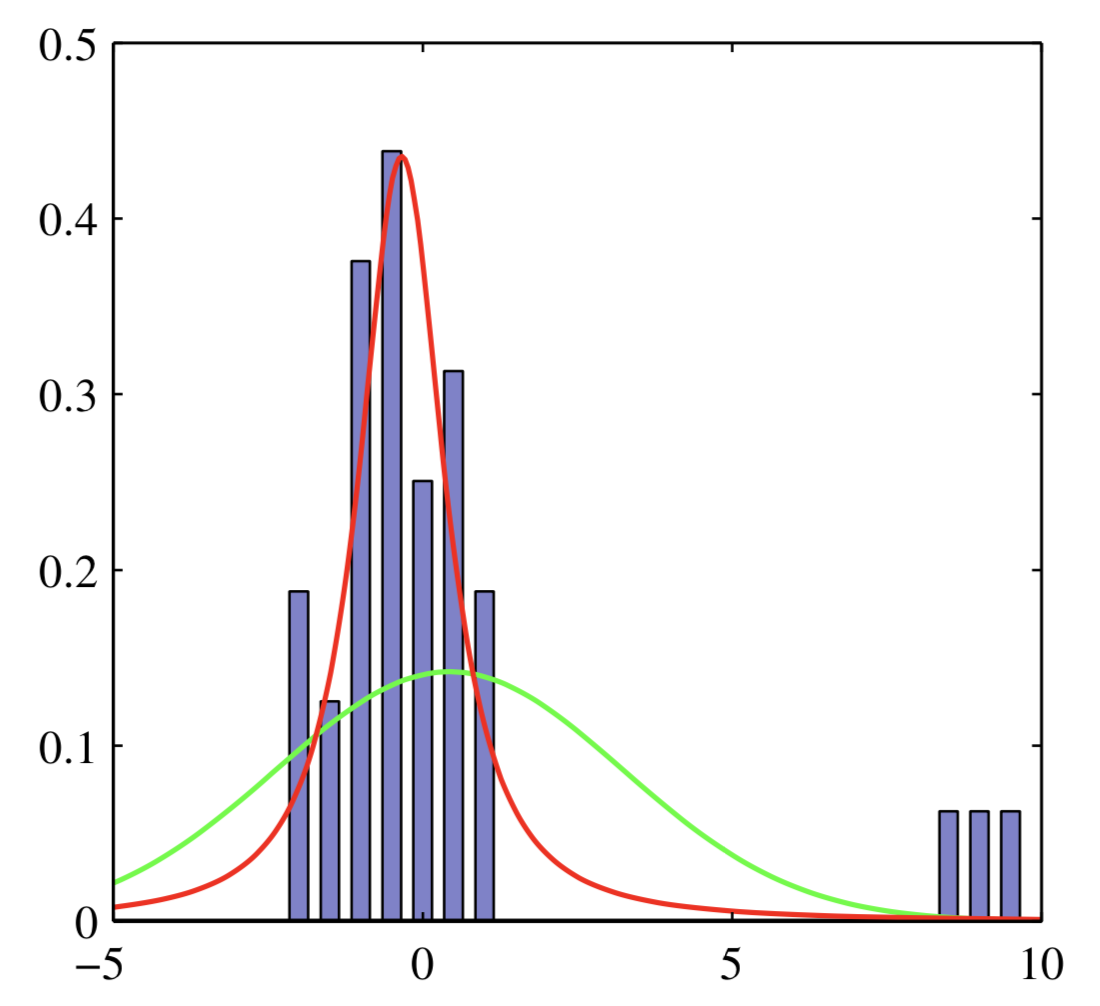
\includegraphics[width=\textwidth]{figures/exponential_families_student_t.png}
			\caption{MLE estimate}
			\label{fig:exponential_families_student_t}
		\end{subfigure}
		\hspace{10mm}
		\begin{subfigure}{0.3\textwidth}
			\centering
			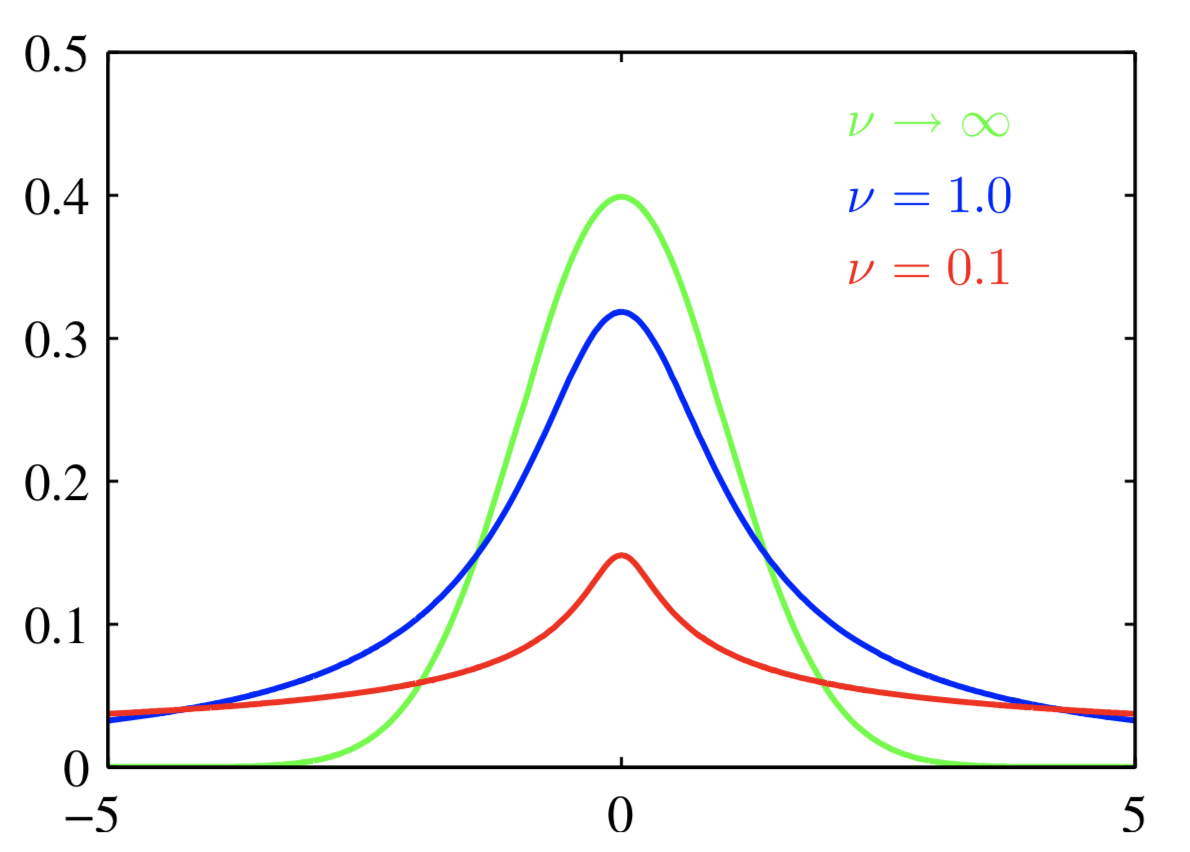
\includegraphics[width=\textwidth]{figures/exponential_families_student_t_nu.png}
			\caption{Effect of parameter $\nu$}
			\label{fig:exponential_families_student_t_nu}
		\end{subfigure}
		\caption{(a) Comparison of MLE solution of Student-t distribution (red) and Gaussian (green). (b) The parameter $\nu$ for fixed $\mu=0$ and $\lambda=1$. For $\nu\to\infty$, }
	\end{figure}
	\item It emerges from a infinite mixture of Gaussians with a fixed mean and the precision (i.e. inverse variance) distributed as a Gamma distribution:
	\begin{enumerate}
		\item Draw precision $\tau \sim \text{Gamma}(a,b)$
		\item Draw $x\sim \mathcal{N}(\mu, \tau^{-1})$
	\end{enumerate}
	Then the resulting $x$ will be distributed according to the Student-t distribution
	$$p(x) \sim \text{St}(x\mid \mu, \lambda=a/b, \nu=2a)$$
	\item By marginalizing out $\tau$, we can derivate the PDF of the student distribution:
	\begin{equation*}
		\begin{split}
			\text{Scalar}\hspace{2mm}&\text{St}(x\mid\mu, \lambda=a/b, \nu=2a) = \frac{b^a}{\Gamma(a)\sqrt{2\pi}}\left(b + \frac{(x-\mu)^2}{2}\right)^{-a-\frac{1}{2}}\Gamma\left(a+\frac{1}{2}\right)\\[8pt]
			\text{d-dimensional}\hspace{2mm} &  \text{St}(\bm{x}\mid\bm{\mu}, \bm{\Sigma}, \nu) = \frac{\Gamma\left(\frac{d}{2} + \frac{\nu}{2}\right)}{\Gamma\left(\frac{d}{2}\right)}\frac{1}{\left(\pi\nu\right)^{d/2}\left|\bm{\Sigma}\right|^{1/2}}\left(1+\nu^{-1}\left(\bm{x}-\bm{\mu}\right)^T \bm{\Sigma}^{-1}\left(\bm{x}-\bm{\mu}\right)\right)^{-\frac{d}{2}-\frac{\nu}{2}}\\
		\end{split}
	\end{equation*}
	\item The parameter $\lambda$ is often called precision, but does not exactly represent the inverse of the variance.
	\item $\nu$ is called the degrees of freedom (see Figure~\ref{fig:exponential_families_student_t_nu}). For $\nu\to\infty$, the student-t distribution becomes a Gaussian $\mathcal{N}(x\vert\mu, \lambda^{-1})$
\end{itemize}
\subsection{Distributions for Binary and Discrete Variables}
\begin{itemize}
	\item In this section, we review common distributions for binary and discrete distributions. We can actually find one-to-one correlations in the binary and categorical space:
	\begin{table}[ht!]
		\centering
		\begin{tabular}{c|c}
			Binary & Discrete\\\hline
			Bernoulli & Categorical\\
			Binomial & Multinomial\\
			Beta & Dirichlet
		\end{tabular}
		\vspace{-5mm}
	\end{table}
\end{itemize}
\subsubsection{Binary}
\begin{description}
	\item[Bernoulli distribution] can be interpreted as a coin flip, and models a single binary outcome:
	$$\text{Bern}(x|\mu)=\mu^{x}(1-\mu)^{1-x}, \hspace{3mm}x\in\{0,1\}$$
	\begin{itemize}
		\item Expectation $\E[x|\mu]=\mu$
		\item Variance $\mathbb{V}\text{ar}[x]=\E[x^2]-\E[x]^2=\mu(1-\mu)$
		\item Maximum likelihood estimate $\mu_{\text{ML}}=\frac{1}{N}\sum_{n=1}^{N} x_n$ (sensitive to overfitting for small dataset)
		\item Exponential family $p(x|\eta)=\sigma(-\eta)\exp(\eta\cdot x), \eta=\ln \frac{\mu}{1-\mu}$
	\end{itemize}

	\item[Binomial distribution] models $N$ i.i.d. Bernoulli experiments, where we define $m$ as $m=\sum_{i=1}^{N}x_i$, i.e. the number of times the outcome is $1$:
	$$\text{Bin}(m|N,\mu)=\frac{N!}{(N-m)!m!}\mu^{m}(1 - \mu)^{N-m}$$	
	\begin{itemize}
		\item Expectation $\E[m]=\sum_{i=1}^{N}\E[x_i]=N\cdot \mu$
		\item Variance $\mathbb{V}\text{ar}[x]=N\cdot \mu(1-\mu)$
		\item Maximum likelihood estimate $\mu_{\text{ML}}=\frac{m}{N}$
		\item Exponential family $p(m|\eta)=\frac{N!}{(N-m)!m!}\cdot \exp(N\log \log 1-\mu) \cdot \exp(m\log\frac{\mu}{1-\mu})$, $\eta=\log \frac{\mu}{1-\mu}$
		\item Conjugate prior: Beta distribution. The posterior is: $\text{Beta}(\mu|a+m,b+N-m)$
	\end{itemize}

	\item[Beta distribution] is the conjugate prior for the binomial distribution
	$$\text{Beta}(\mu|a,b)=\frac{\Gamma(a+b)}{\Gamma(a)\Gamma(b)}\mu^{a-1}(1-\mu)^{b-1}$$
	\begin{itemize}
		\item Expectation $\E[\mu]=\frac{a}{a+b}$
		\item Variance $\mathbb{V}\text{ar}[x]=\frac{ab}{(a+b)^2(a+b+1)}$
		\item Exponential family: see Appendix
	\end{itemize}
\end{description}
\subsubsection{Discrete}
\begin{description}
	\item[Categorical distribution] considers a single sample, and assign each category a different probability. The input $\bm{x}$ is a one-hot vector.
	$$\text{Cat}(\bm{x}|\bm{\mu})=\prod_{k=1}^{K}\mu_k^{x_k}=\mu_{x_k}, \hspace{3mm}\sum_k \mu_k = 1$$
	 \begin{itemize}
	 	\item Expectation $\E[\bm{x}]=\bm{\mu}$
	 	\item Covariance $\text{Cov}[\bm{x}]=\text{diag}(\bm{\mu}(1-\bm{\mu}))$
	 	\item Maximum likelihood estimate  $\bm{\mu}_{\text{ML}}=\frac{1}{N}\sum_{i=1}^{N} \bm{x}$
	 	\item Exponential family $p(\bm{x}|\bm{\eta})=\frac{1}{1+\sum_{k=1}^{K-1}\exp(\eta_k)}\cdot \exp(\bm{\eta}^T\bm{x})$, $\eta_k=\ln\frac{\mu_k}{1-\sum_{j=1}^{K-1}\mu_j}$
	 \end{itemize}
	\item[Multinomial distribution] takes $N$ i.i.d. categorical observations into account, where $m_k=\sum_{n=1}^{N} x_{nk}$.
	$$\text{Mult}(m_1,...,m_K|N,\bm{\mu})=\frac{N!}{\prod_{k=1}^{K}m_k!}\prod_{k=1}^{K} \mu_{k}^{m_k}$$
	\begin{itemize}
		\item Expectation: $\E[\bm{x}]=N\cdot \mu$
		\item Covariance: $\text{Cov}[\bm{x},\bm{x}]=N(\text{diag}(\bm{\mu})-\bm{\mu}\bm{\mu}^T)$
		\item Maximum likelihood estimation: $\bm{\mu}_{\text{ML}}=\frac{\bm{m}}{N}$
		\item Exponential family: see Appendix
	\end{itemize}
	\item[Dirichlet distribution] is the conjugate prior for multinomial
	$$\text{Dir}(\bm{\mu}|\bm{\alpha})=\frac{\Gamma(\sum_k \alpha_k)}{\prod_k
	\Gamma(\alpha_k)} \prod_{k=1}^{K}\mu_k^{\alpha_k-1}$$
	\begin{itemize}
		\item Expectation $\E[\bm{x}]=\frac{1}{\sum_k \alpha_k}\bm{\alpha}$
		\item Covariance $\text{Cov}[\bm{x}]=-\frac{1}{\sum_k \alpha_k + 1}\bm{\alpha}\bm{\alpha}^T$
		\item Exponential family: see Appendix
	\end{itemize}
\end{description}
\subsection{Independent Component Analysis}
\begin{itemize}
	\item Independent Component Analysis (ICA) tries to reconstruct source signals from linearly mixed measurements. For example, for two sources $S(t)=\begin{bmatrix}
	S_1(t)\\S_2(t)
	\end{bmatrix}$, we assume to have the measurements:
	$$X(t)=\begin{bmatrix}
	X_1(t)\\X_2(t)
	\end{bmatrix} = \begin{bmatrix}
	\alpha_1 S_1(t) + \beta_1 S_2(t)\\\alpha_2 S_2(t) + \beta_2 S_2(t)
	\end{bmatrix}$$
	The goal is now to find the parameter matrix
	$$\bm{A}=\begin{bmatrix}
	\alpha_1 & \beta_1\\ \alpha_2 & \beta_2
	\end{bmatrix}$$
	to reconstruct our signals $S(t)$ from the measurements $\bm{X}(t)=\bm{A}\bm{S}(t)$
	\item Note that we can only reconstruct $S(t)$ up to permutation and scaling/multiplicative factors as these give the same result
	\item As we assume the sources to be independent, we can write the joint probability distribution as:
	$$p(S_1,...,S_I)=\prod_{i=1}^{I}p(S_i)$$
	One crucial element of ICA is that these prior distributions need to be designed by the user. This requires pre-knowledge of how the source signals can look like (e.g. Gaussian, bounded Uniform, etc.). The performance of the algorithm depend on this design choice, and can lead to ICA failing if the prior has a very different distribution than points in the sources.
	\item We will again use a maximum likelihood  approach where we try to increase the probability of the observed data, which can be derived as:
	$$\ln p(\bm{x}|\bm{A})=\ln |\det \bm{A}| + \frac{1}{N}\sum_{n=1}^{N}\sum_{i=1}^{I}\ln p_i\left(\sum_{j=1}^{I} \left(A^{-1}\right)_{ij} x^{(n)}_j\right)$$
	For simplicity, we replace $\bm{A}^{-1}=\bm{W}$, and aim to learn $\bm{W}$ which is slightly easier.
	\item We take now the derivative with respect to $\bm{W}$, and end up with the following expression:
	$$\bm{W}^{t+1}=\bm{W}^{t} + \alpha \cdot \frac{1}{N}\sum_{n=1}^{N}\left(\nabla_{\bm{S}} \log p(\bm{S})\Big\vert_{S=S_n}\bm{S}_n^T+\bm{I}\right)\bm{W}$$
	where we estimate $\bm{S}=\bm{W}\bm{X}$. In addition, we see here that what we actually need from our prior is the derivative of its log. Hence, the prior is mostly designed to have a simple form of $\Phi_i=\frac{\partial \ln p_i(a_i)}{\partial a_i}$.
	\item We can slightly simplify the gradient calculation by splitting it into multiple parts. Summarizing the full algorithm, we get:
	\begin{tcolorbox}[colback=white!80!gray,colframe=gray!75!black,title=Independent Component Analysis]
		\begin{algorithm}[H]
			\SetAlgoLined
			Choose prior and calculate log derivative $\Phi_i=\frac{\partial \ln p_i(a_i)}{\partial a_i}$\;
			Set learning rate $\eta$\;
			Initialize $\bm{W}=\bm{A}^{-1}$\;
			\While{$\nabla \bm{W}^{(t)} > \epsilon$}{
				Let $\hat{\bm{S}}=\bm{W}\bm{X}$ be the current estimate of $\bm{S}$\;
				Let $\bm{Z}_i=\Phi_i(\hat{\bm{S}}_i)$\;
				Let $\bm{X}' = \bm{W}^T\hat{\bm{S}}$\;
				Calculate the gradients $\nabla \bm{W}^{(t)}= \bm{W}^{(t)} + \frac{1}{N}\left[ \bm{Z}{\bm{X}'}^T\right]$\;
				Apply gradient with learning rate $\bm{W}^{(t+1)}=\bm{W}^{(t)}+\eta \nabla \bm{W}^{(t)}$\;
			}
			Reconstruct signals $\bm{S}_n=\bm{W}\bm{X}_n$\;
		\end{algorithm}
	\end{tcolorbox} 
	\item One issue with ICA is that the signals are not allowed to be Gaussian. If this would be the case, we can not reconstruct the signal up to rotation as Gaussians are rotation invariant. Hence, the signals will be messed up although we find an optimum
\end{itemize}
\subsection{Information theory}
\begin{itemize}
	\item The information of an event $A$ can be measured by:
	\begin{equation*}
		\begin{split}
			h(A) & = -\log_2 p(A)\hspace{4mm}\text{(in bits)}\\
			& = - \ln p(A)\hspace{4mm}\text{(in nats)}
		\end{split}
	\end{equation*}
	\item An important measurement of a distribution in information theory is the Shannon entropy, which can be interpreted as the expected information of an event according to the distribution $p$:
	\begin{equation*}
		\tcbox[nobeforeafter]{\(
			H(X) = -\sum_{x\in D_x} p(x)\log_2 p(x)
		\)}
	\end{equation*}
	In case we have $N$ independent events, the entropy is the sum of the single entropy of each of the $N$ events.
	\item The entropy can also be defined for continuous space. It is then referred to as the differential entropy:
	$$H(\bm{x})=-\int p(\bm{x})\log_2 p(\bm{x})d\bm{x}$$
	\item We can also define conditional entropy, which is as follows:
	\begin{equation*}
	\tcbox[nobeforeafter]{\(
		H(\bm{x}|\bm{y}) = -\int p(\bm{x})\left[\int p(\bm{y}|\bm{x})\ln p(\bm{y}|\bm{x})d\bm{y}\right]d\bm{x}
		\)}
	\end{equation*}
	with the property $H(\bm{x},\bm{y})=H(\bm{x})+H(\bm{y}|\bm{x})=H(\bm{y})+H(\bm{x}|\bm{y})$
	\item Another well-known measurement is the Kullback-Leiber divergence (also referred to as relative entropy):
	\begin{equation*}
		\tcbox[nobeforeafter]{\(
			\text{KL}(p(\bm{x})||q(\bm{x})) = -\int p(\bm{x})\frac{q(\bm{x})}{p(\bm{x})}d\bm{x}
		\)}
	\end{equation*}
	Some properties of this divergence are:
	\begin{itemize}
		\item Always positive: $\text{KL}(p||q)\geq 0$
		\item If $\text{KL}(p||q) = 0$, then $p=q$ (if $p$,$q$ are sufficient regular, i.e. strictly positive and integral defined)
		\item The triangular inequality does not hold for KL, thus it is not a distance measure: 
		
		$\text{KL}(p||q)+\text{KL}(q||r)\not\geq \text{KL}(p||r)$
	\end{itemize}
	\item Mutual information describes the amount of information that is shared among $x$ and $y$:
	\begin{equation*}
		\tcbox[nobeforeafter]{\(
			I(\bm{x};\bm{y}) = \text{KL}(p(\bm{x},\bm{y})||p(\bm{x}),p(\bm{y})) = H(\bm{x})-H(\bm{x}|\bm{y}) = H(\bm{y}) - H(\bm{y}|\bm{x})
		\)}
	\end{equation*}
	In other words, how much information about $y$ do I get by observing $x$. In a diagram, mutual information can be visualized as follows:
	\begin{figure}[ht!]
		\centering
		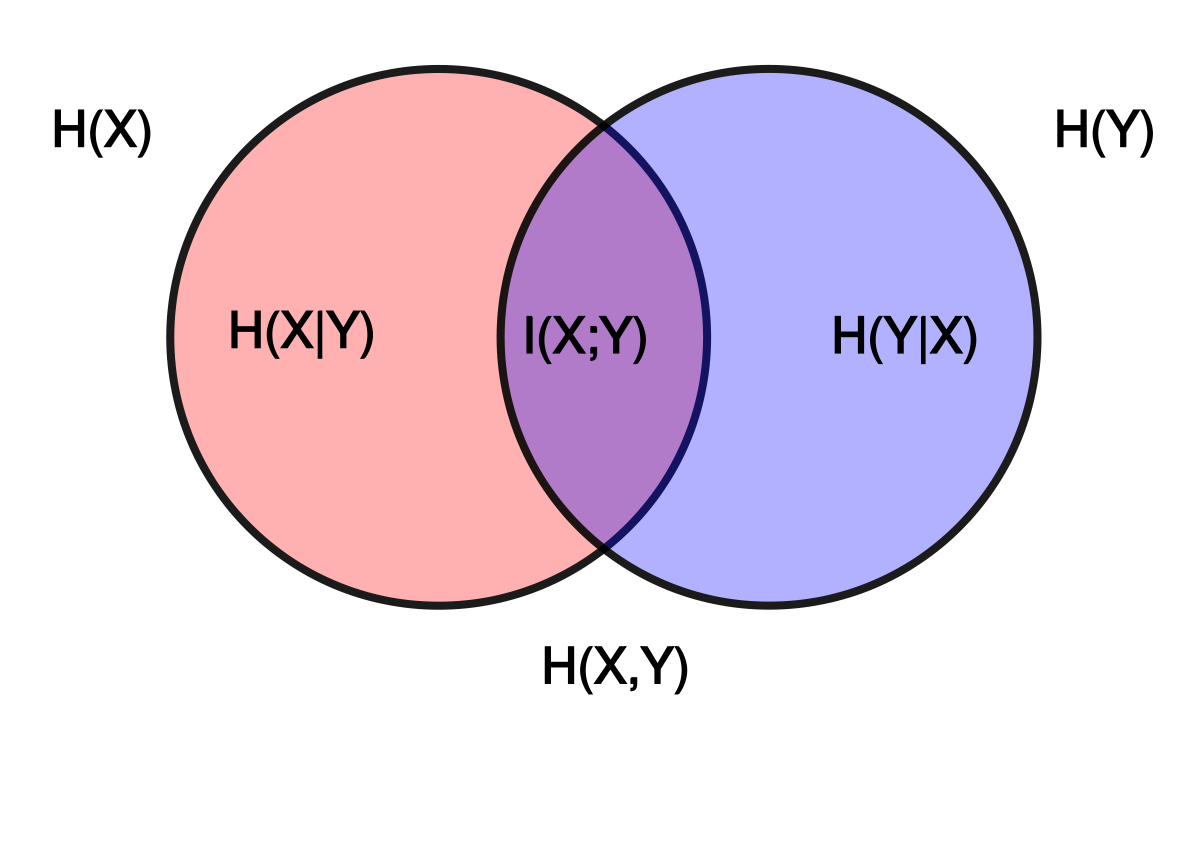
\includegraphics[width=0.3\textwidth]{figures/information_theory_mutual_information.png}
		\caption{Visualizing the relationship between mutual information and entropy.}
	\end{figure}
\end{itemize}
